\chapter{Ferramentas}

Este capítulo introduz as ferramentas que serão utilizadas ao longo do desenvolvimento. Descreve-se aqui o OpenCV e suas funcionalidades principais, dando ênfase em funções que fazem parte da solução. Também são demonstradas as bibliotecas de OCR GOCR \cite{GOCR}, OCRAD \cite{OCRAD} e Tesseract \cite{tesseract-ocr}.

\section{O OpenCV}

O OpenCV é uma biblioteca de visão computacional disponível de forma gratuita, escrita na linguagem de programação C e \cpp, sendo ela multiplataforma podendo ser usada em qualquer distribuição Linux, Windows e Mac OS X. O OpenCV pode ser integrado em linguagens como o Python, Ruby, Matlab, C e \cpp, dentre outras \cite{learningopencv}. Ele teve início como um projeto de pesquisa da Intel \cite{intel} no ano de 1998, ficando disponível com licença BSD em 2000. Foi registrado que o download dessa biblioteca foi efetuado mais de três milhões de vezes até 2012 \cite{pulli2012real}, e até hoje vem crescendo e tem sido usado por profissionais da área, professores e estudantes.

Projetado para ter um bom desempenho diante de aplicações em tempo real, o OpenCV trabalha bem com processadores Intel. A própria empresa vende determinadas bibliotecas extras para melhorias em relação ao desempenho do OpenCV. Um dos principais objetivos do OpenCV é providenciar uma infraestrutura de visão computacional que auxilia profissionais específicos da área, professores e estudantes a desenvolverem sistemas sofisticados com simplicidade e eficiência, disponibilizando mais de quinhentas funções como por exemplo, inspeção de produtos de fábrica, imagem médica, segurança, interface para usuários, calibração de câmera, visão estéreo e robótica \cite{learningopencv}. 

\subsection{Funcionalidades do OpenCV}

Algumas das funcionalidades do OpenCV serão exibidas nesta sub-sessão, todos os códigos deste e de outros capítulos estão na linguagem Python 2.7.2. Como analisado, existem mais de quinhentas funções no OpenCV, contudo, serão analisadas apenas algumas funções gerais de processamento de imagens e um exemplo de aplicação.

\subsection{Dilatação e Erosão}	
O OpenCV disponibiliza funções de filtros que serão abordados na sessão de desenvolvimento, um destes é conhecido como dilatação (\autoref{fig:dilatacao}). De acordo com os autores \cite{oge1999processamento} para compreender a fórmula matemática de dilatação faz-se necessário compreender também os seguintes conceitos:

\begin{figure}[htbp]
\caption{\label{fig:dilatacao}Demonstração do efeito de dilatação sobre um \textit{pixel}}
\begin{center}
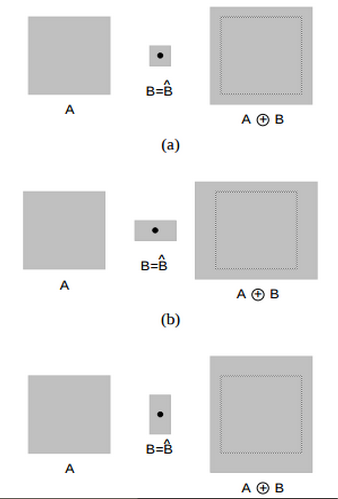
\includegraphics[width=.3\textwidth]{figuras/f1c3.png}
\end{center}
\legend{Fonte: \citeonline{oge1999processamento}}
\end{figure} 

Sejam $A$ e $B$ conjuntos no espaço $ Z^2 $ onde respectivamente $A = (a1 , a2)$ e $B = (b1 , b2)$, e seja $\emptyset$ o conjunto vazio. A denotação $(A)_x$ é definida pela translação de $A$ por um $x$ qualquer onde $x = (x1 ,  x2)$. Tem-se:
\[
(A)_x = \{c | c = a + x\}, \mbox{para~} a \in A
\]
Isso quer dizer que, se $x$ supostamente fosse igual ao ponto $(1,2)$ e $A$ fosse igual ao ponto $(3,3)$ a translação de $A$ por $x$ seria igual ao ponto $(4,5)$. Todos os \textit{pixels} se deslocariam de $A$ até $x$, resultando no ponto encontrado ao fim da equação.

A reflexão de $B$ é dada por:
\[
\hat{B} = \{x | x = -b \mbox{ para } b \in B\}
\]
Logo, a reflexão de $B$ trata-se da rotação de 180\textordmasculine \hspace{} em relação a origem.

O Complemento de $A$ é:
\[
A^c = \{x | x \not \in A\}
\]

Ou seja, o complemento de $A$ são os pixels que não pertencem a $A$, em uma imagem binária (preto e branco) corresponderia aos \textit{pixels} brancos da figura caso o objeto principal fosse em preto como na \autoref{fig:filtros2}(b).

\begin{figure}[htbp]
\caption{\label{fig:filtros2}Filtros de dilatação e erosão sobre uma imagem}
\begin{center}
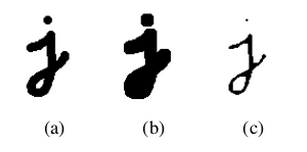
\includegraphics[width=.5\textwidth]{figuras/f3c3.png}
\end{center}
\legend{Fonte: \citeonline{caap}}
\end{figure} 

A diferença entre $A$ e $B$ é definida por:
\[
A - B = \{x | x \in A,x \not \in B\} = A \cap B^c
\]
Portanto, sendo a diferença de $A$ e $B$ igual a intersecção de $A$ por complemento de $B$, essa diferença será os pontos em comum de $A$ e complemento de $B$. Com os conceitos apresentados compreendidos, segue a fórmula da dilatação:

\[A \oplus B = \{x|(\hat{B})_x \cap A \notin \emptyset\}\]

\noindent onde que $A$ representa a imagem a ser operada, e $B$ é um segundo conjunto de pixels, de uma forma que opera sobre os pixels de A para produzir o resultado. O conjunto B é chamado de elemento estruturante. A dilatação de $A$ por $B$ é o conjunto de todos os deslocamentos de $x$ tais que $A$ sobreponham-se em pelo menos um elemento não nulo.


No OpenCV, a dilatação pode ser aplicada de maneira simples, dando apenas duas entradas de dados, sendo elas a própria imagem e o kernel. O Kernel\footnote{Matriz de convolução utilizada para borrar, controlar nitidez dentre outras funções. No caso desse trabalho, define a expessura da dilatação e da erosão \cite{shapiro2001computer}.} de maneira bem resumida definirá a espessura do resultado final, basicamente é responsável por definir o quanto será dilatada a imagem \cite{opencv}. O Código 1 é um código de dilatação de uma imagem, onde inicia-se importando as bibliotecas OpenCV e Numpy, respectivamente cv2 e np. Após a importação das bibliotecas principais, uma variável chamada ``img'' utiliza a função \textit{imread} do OpenCV, que apenas faz uma leitura da imagem ``j.png'' em escala de cinza, definida pelo parâmetro ``0''. Assim define-se o \textit{kernel} e por fim a dilatação, feita através da função \textit{dilate} também do OpenCV. Segue o código comentado:

\lstinputlisting[language=python,caption={Dilatação de uma imagem},label=mediapy]{codigos/dilate.py}

A erosão é o inverso da dilatação. Se por um lado o efeito da dilatação adiciona pixels a um objeto, a erosão retira \cite{parker10@algorithms}. O efeito da erosão pode ser observado na \autoref{fig:filtros2}(c). A fórmula matemática do efeito de erosão é:

\[ A \ominus B = \{c|(B)_c \subseteq A\} \]

O conjunto $A \ominus B$ é o conjunto de translações de B que se alinham sobre um conjunto de pixels pretos em $A$. Isto significa que nem todas as translações devem ser consideradas, mas apenas aquelas que, sobrepõe a origem de $B$ em um dos membros de $A$. \cite{parker10@algorithms}. Abaixo segue o Código 2, sendo ele muito semelhante ao Código 1, apenas diferenciando-se na aplicação final da função do OpenCV \textit{erode} no lugar da função \textit{dilate}.

\lstinputlisting[language=python,caption={Erosão de uma imagem com base na fonte},label=mediapy]{codigos/erosion.py}

Observa-se que as funções de dilatação e erosão são aplicadas de forma praticamente idêntica. Não existe apenas uma forma de aplicar dilatação e erosão, pelo contrário, outras fórmulas dependente da situação podem ser encontradas \cite{parker10@algorithms}, entretanto de forma geral estas apresentadas são base para compreensão do tema.


\subsection{Limiarização - Thresholding}

Limiarização\footnote{Alguns autores traduzem o termo como \textit{binarização}} é um método de segmentação baseado em similaridade de níveis de cinza, buscando extrair objetos de interesse mediante a definição de um limiar $T$ que separa os agrupamentos de níveis de cinza da imagem. A segmentação se dá varrendo a imagem, pixel a pixel, e rotulando cada pixel como sendo do objeto ou do fundo, em função da relação entre o valor do pixel e o valor do limiar \cite{IntroProcessDigIMG}. Limiarização é computacionalmente barato e rápido, é o método de segmentação mais antigo e ainda é amplamente utilizado em aplicações simples. Pode facilmente ser usado em tempo real. Limiarização é a transformação da imagem $f$ para obter como saída a imagem $g$, como pode ser visto na fórmula abaixo \cite{sonka2014image}:

\[
g(i,j) = 1 \mbox{~para~} f(i,j) > T 
\]
\[
g(i,j) = 0 \mbox{~para~} f(i,j) \leq T
\]

Em que $T$ é o limiar que é definido conforme o histograma da imagem e também de acordo com quantos objetos se quer extrair da imagem, e os pontos $g$ e $f$ representam pixels da imagem $g$ e da imagem $f$. Quando $g(i,j)$ é igual a $0$, caracteriza o fundo da imagem, e quando $g(i,j)$ é igual a $1$, caracteriza-se o objeto \cite{sonka2014image}.

Este método de limiarização apresentado, é mais simples. Há outros métodos de limiarização, basicamente a diferença entre eles é a forma ou solução para encontrar o limiar $T$. O OpenCV disponibiliza cinco tipos diferentes de limiarização que são demonstrados no Código 3 e na \autoref{fig:limiar} \cite{opencv}. Não serão explicados aqui detalhes a respeito de todas as limiarizações, apenas uma pequena demonstração de cada uma. 

Para que os códigos apresentados no Código 3 façam sentido, faz-se necessário o conhecimento básico do que é a biblioteca Matplotlib. Matplotlib é uma biblioteca de geração de gráficos bidimensional Python, que produz figuras de qualidade de publicação, em uma variedade de formatos e em várias plataformas. O Matplotlib permite gerar gráficos, histogramas, espectros de potência, gráficos de barras, gráficos de dispersão e outras funções \cite{Hunter:2007}. 

O Código 3 possui além das importações já comentadas anteriormente, a importação do matplotlib na linha 6. A leitura de uma imagem chamada ``31.jpg'' é feita, e então da linha 9 até a linha 13 são aplicadas as funções de limiarização disponíveis no OpenCV. Os valores 127 e 255 são \textit{limiares} utilizados de forma geral por padrão para aplicar limiarização em imagens. O matplot é utilizado apenas para apresentar essas imagens uma ao lado da outra como pode ser verificado na \autoref{fig:limiar}. Na linha 15 do Código 3, uma lista de nomes são agregados a uma lista de cada imagem \textit{limiarizada}, e ambos são apresentados através do MatPlot nos comandos da linha 18 até a 22. Segue o Código 3:

\lstinputlisting[language=python,caption={Thresholding em uma placa},label=mediapy]{codigos/thresholding.py}

\begin{figure}[htbp]
\caption{\label{fig:limiar}Thresholding(Limiarização) sobre uma imagem de uma placa}
\begin{center}
	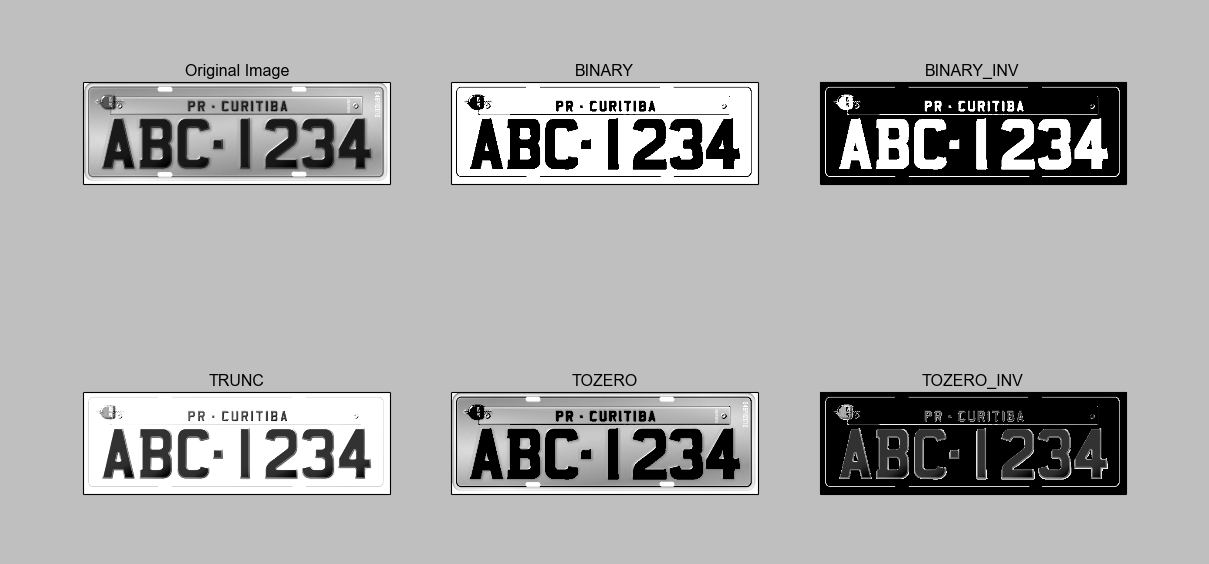
\includegraphics[width=.9\textwidth]{figuras/f2c3.png}
\end{center}
\legend{Fonte: o autor}
\end{figure} 
 
\subsection{Detecção de bordas, Histogramas e Detecção de cores}

Detecção de bordas Canny é um dos algoritmos de detecção de borda que o OpenCV dispõe, e será usado aqui como exemplo embora existam outros algoritmos que possam ser tão úteis quanto ele. Ele foi desenvolvido por John F. Canny em 1986. É um algoritmo que passa por alguns estágios antes de sua solução final. Iniciando pela remoção de ruídos, encontrando a intensidade do gradiente da imagem, removendo pixels indesejados e finalmente encontrando as bordas \cite{opencv}. 

Para utilizar o algoritmo de Canny, basta fazer uso da função ``cv2.Canny'' como feito na linha 6 do Código 4. Os valores 100 e 200 observados na linha 6, são também valores utilizados por padrão. A \autoref{fig:deteccao_bordas} representa o resultado do Código 4 sobre uma imagem.

\lstinputlisting[language=python,caption={Detecção de bordas Canny, resultado representado pela Figura 9},label=mediapy]{codigos/deteccaobordas.py}

\begin{figure}[htbp]
\caption{\label{fig:deteccao_bordas}Resultado do código de Detecção de bordas sobre uma imagem de uma placa}
\begin{center}
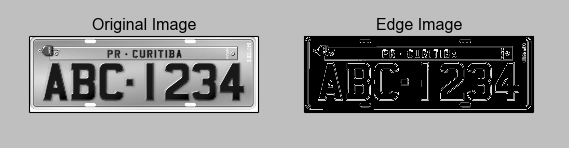
\includegraphics[width=.9\textwidth]{figuras/f4c3.png}
\end{center}
\legend{Fonte: o autor}
\end{figure} 

Além dessa função de detecção de bordas o OpenCV disponibiliza visualização de histogramas, que são lidos através da biblioteca MatPlotLib. O histograma é uma das mais comuns formas de representação das distribuições de pixel em uma imagem. Quando observado é possível obter instantâneamente noções das características da imagem em questão, podendo inferir informações relevantes, como a intensidade das cores \cite{neta2008limiarizaccao}.

O Código 5 é um exemplo de código utilizando a mesma placa da \autoref{fig:deteccao_bordas} e sequencialmente a \autoref{fig:resultado_histograma} apresenta o resultado do código. É possível verificar na linha 6 que para apresentar o histograma basta utilizar a função \textit{hist} da MatPlotLib:


\lstinputlisting[language=python,caption={Histograma, resultado representado pela Figura 10},label=mediapy]{codigos/histogramas.py}

\begin{figure}[htbp]
\caption{\label{fig:resultado_histograma}Resultado do código de histrograma}
\begin{center}
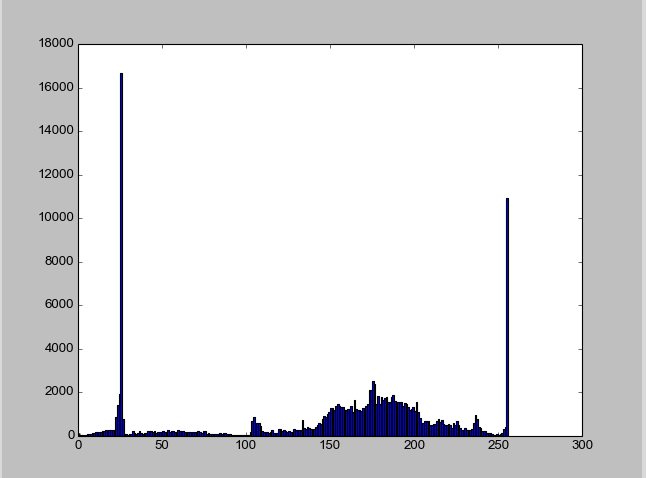
\includegraphics[width=.9\textwidth]{figuras/f5c3.png}
\end{center}
\legend{Fonte: o autor}
\end{figure} 

Para concluir a sessão do OpenCV, será mostrado uma pequena aplicação que destaca apenas a cor azul de objetos que possam estar em frente a câmera. Pode-se notar que neste caso não é aberta uma imagem como entrada, mas sim captura direta da câmera, ou seja, tempo real. Este código não trabalha com o padrão RGB(\textit{red green blue}) de cores, mas sim o padrão conhecido como HSV(\textit{hue saturation value}). 

Na linha 4 do Código 6 é iniciada a leitura da câmera, e então na linha 6 é criado um laço sem finalização. A linha 9 captura cada \textit{frame} da câmera, e em na linha 12 é convertido para o padrão HSV. As linhas 15 e 16 definem os valores da cor azul, e na linha 19 é aplicada a função inRange para extrair apenas essa cor. A partir da linha 22 são apenas utilizados códigos para a apresentação na tela. O representação do resultado está na \autoref{fig:deteccao_cor}.

\lstinputlisting[language=python,caption={Encontrando objetos da cor azul, resultado representado pela Figura 11},label=mediapy]{codigos/findblue.py}

\begin{figure}[htbp]
\caption{\label{fig:deteccao_cor}Resultado do código de detecção de cor azul}
\begin{center}
	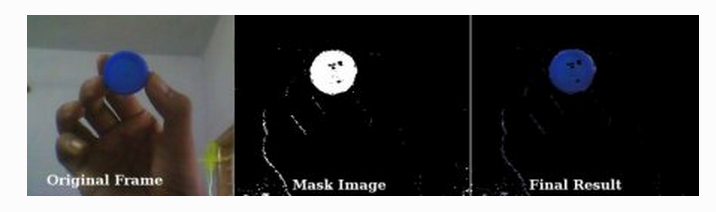
\includegraphics[width=.9\textwidth]{figuras/f6c3.png}
\end{center}
\legend{Fonte: \citeonline{opencv}}
\end{figure} 

\section{O GOCR e o OCRAD}

Nos dois capítulos anteriores, já foram identificadas as funções de uma OCR, e também foram citados os nomes de algumas bibliotecas OCR. O GOCR e o OCRAD sendo algumas dessas bibliotecas compõe parte importante neste trabalho, haja visto que trata-se da comparação de uma solução que não possui treinamento de reconhecimento de novos caracteres, utilizando ambas as bibliotecas, e uma solução utilizando o Tesseract(especificado na próxima sessão) com o uso de treinamento. 

O GOCR é um motor OCR desenvolvido sob a Licença Pública GNU. Ele converte imagens digitalizadas de texto em arquivos de texto manipuláveis. Joerg Schulenburg foi quem criou a ferramenta, e passou a liderar uma equipe de desenvolvedores que procuraram melhorar a qualidade do GOCR. O GOCR pode ser usado em diferentes sistemas operacionais e arquiteturas. Ele pode abrir muitos formatos de imagem diferentes. Sua atualização mais recente é de 05/03/2013, sendo nomeada de "GOCR 0.50", estando disponível para download no site oficial \cite{GOCR}.

O OCRAD também é um motor OCR de licença GNU, com base em um método de extração de características. A leitura de imagens são pelas extensões PBM(bitmap), pgm(escala de cinza) ou ppm(colorida) e extrai o texto nos formatos byte ou UTF-8. Também inclui um analisador de layout capaz de separar as colunas ou blocos de texto normalmente encontrados nas páginas impressas. Ocrad pode ser usado como um aplicativo de console autônomo, ou como um \textit{backend} para outros programas. Assim como o GOCR, também pode-se contribuir para o melhoramento desse programa\cite{OCRAD}. O OCRAD também tem um manual online em sua página oficial.

\section{Tesseract}

Tesseract é o motor OCR de licença gratuita desenvolvido pela HP(Hewlett-Packard) \cite{Hewlett-Packard} por volta de 1984 e 1994. Foi modificado e melhorado em 1995 tendo bons resultados. Tornou-se verdadeiramente licença gratuita em 2005. Hoje pertencente oficialmente a Google, o Tesseract possui suporte a diversas linguagens, tendo que ser treinado para o caso específico no qual esteja sendo submetido, para assim gerar os resultados desejados\cite{patel2012optical}.

\subsection{Conclusão}

Nesse Capítulo foram apresentadas as ferramentas que serão utilizadas no Capítulo 4. Alguns exemplos práticos foram citados e demonstrados. Cada exemplo possui um código e uma imagem que demonstra o respectivo resultado.